\documentclass[]{book}
\usepackage{lmodern}
\usepackage{amssymb,amsmath}
\usepackage{ifxetex,ifluatex}
\usepackage{fixltx2e} % provides \textsubscript
\ifnum 0\ifxetex 1\fi\ifluatex 1\fi=0 % if pdftex
  \usepackage[T1]{fontenc}
  \usepackage[utf8]{inputenc}
\else % if luatex or xelatex
  \ifxetex
    \usepackage{mathspec}
  \else
    \usepackage{fontspec}
  \fi
  \defaultfontfeatures{Ligatures=TeX,Scale=MatchLowercase}
\fi
% use upquote if available, for straight quotes in verbatim environments
\IfFileExists{upquote.sty}{\usepackage{upquote}}{}
% use microtype if available
\IfFileExists{microtype.sty}{%
\usepackage{microtype}
\UseMicrotypeSet[protrusion]{basicmath} % disable protrusion for tt fonts
}{}
\usepackage[left=3cm,right=3cm,top=2cm,bottom=2cm]{geometry}
\usepackage{hyperref}
\hypersetup{unicode=true,
            pdftitle={Patterns and Trends in Environmental Data},
            pdfauthor={Patrick Laube and Nils Ratnaweera},
            pdfborder={0 0 0},
            breaklinks=true}
\urlstyle{same}  % don't use monospace font for urls
\usepackage{color}
\usepackage{fancyvrb}
\newcommand{\VerbBar}{|}
\newcommand{\VERB}{\Verb[commandchars=\\\{\}]}
\DefineVerbatimEnvironment{Highlighting}{Verbatim}{commandchars=\\\{\}}
% Add ',fontsize=\small' for more characters per line
\usepackage{framed}
\definecolor{shadecolor}{RGB}{248,248,248}
\newenvironment{Shaded}{\begin{snugshade}}{\end{snugshade}}
\newcommand{\AlertTok}[1]{\textcolor[rgb]{0.94,0.16,0.16}{#1}}
\newcommand{\AnnotationTok}[1]{\textcolor[rgb]{0.56,0.35,0.01}{\textbf{\textit{#1}}}}
\newcommand{\AttributeTok}[1]{\textcolor[rgb]{0.77,0.63,0.00}{#1}}
\newcommand{\BaseNTok}[1]{\textcolor[rgb]{0.00,0.00,0.81}{#1}}
\newcommand{\BuiltInTok}[1]{#1}
\newcommand{\CharTok}[1]{\textcolor[rgb]{0.31,0.60,0.02}{#1}}
\newcommand{\CommentTok}[1]{\textcolor[rgb]{0.56,0.35,0.01}{\textit{#1}}}
\newcommand{\CommentVarTok}[1]{\textcolor[rgb]{0.56,0.35,0.01}{\textbf{\textit{#1}}}}
\newcommand{\ConstantTok}[1]{\textcolor[rgb]{0.00,0.00,0.00}{#1}}
\newcommand{\ControlFlowTok}[1]{\textcolor[rgb]{0.13,0.29,0.53}{\textbf{#1}}}
\newcommand{\DataTypeTok}[1]{\textcolor[rgb]{0.13,0.29,0.53}{#1}}
\newcommand{\DecValTok}[1]{\textcolor[rgb]{0.00,0.00,0.81}{#1}}
\newcommand{\DocumentationTok}[1]{\textcolor[rgb]{0.56,0.35,0.01}{\textbf{\textit{#1}}}}
\newcommand{\ErrorTok}[1]{\textcolor[rgb]{0.64,0.00,0.00}{\textbf{#1}}}
\newcommand{\ExtensionTok}[1]{#1}
\newcommand{\FloatTok}[1]{\textcolor[rgb]{0.00,0.00,0.81}{#1}}
\newcommand{\FunctionTok}[1]{\textcolor[rgb]{0.00,0.00,0.00}{#1}}
\newcommand{\ImportTok}[1]{#1}
\newcommand{\InformationTok}[1]{\textcolor[rgb]{0.56,0.35,0.01}{\textbf{\textit{#1}}}}
\newcommand{\KeywordTok}[1]{\textcolor[rgb]{0.13,0.29,0.53}{\textbf{#1}}}
\newcommand{\NormalTok}[1]{#1}
\newcommand{\OperatorTok}[1]{\textcolor[rgb]{0.81,0.36,0.00}{\textbf{#1}}}
\newcommand{\OtherTok}[1]{\textcolor[rgb]{0.56,0.35,0.01}{#1}}
\newcommand{\PreprocessorTok}[1]{\textcolor[rgb]{0.56,0.35,0.01}{\textit{#1}}}
\newcommand{\RegionMarkerTok}[1]{#1}
\newcommand{\SpecialCharTok}[1]{\textcolor[rgb]{0.00,0.00,0.00}{#1}}
\newcommand{\SpecialStringTok}[1]{\textcolor[rgb]{0.31,0.60,0.02}{#1}}
\newcommand{\StringTok}[1]{\textcolor[rgb]{0.31,0.60,0.02}{#1}}
\newcommand{\VariableTok}[1]{\textcolor[rgb]{0.00,0.00,0.00}{#1}}
\newcommand{\VerbatimStringTok}[1]{\textcolor[rgb]{0.31,0.60,0.02}{#1}}
\newcommand{\WarningTok}[1]{\textcolor[rgb]{0.56,0.35,0.01}{\textbf{\textit{#1}}}}
\usepackage{longtable,booktabs}
\usepackage{graphicx,grffile}
\makeatletter
\def\maxwidth{\ifdim\Gin@nat@width>\linewidth\linewidth\else\Gin@nat@width\fi}
\def\maxheight{\ifdim\Gin@nat@height>\textheight\textheight\else\Gin@nat@height\fi}
\makeatother
% Scale images if necessary, so that they will not overflow the page
% margins by default, and it is still possible to overwrite the defaults
% using explicit options in \includegraphics[width, height, ...]{}
\setkeys{Gin}{width=\maxwidth,height=\maxheight,keepaspectratio}
\IfFileExists{parskip.sty}{%
\usepackage{parskip}
}{% else
\setlength{\parindent}{0pt}
\setlength{\parskip}{6pt plus 2pt minus 1pt}
}
\setlength{\emergencystretch}{3em}  % prevent overfull lines
\providecommand{\tightlist}{%
  \setlength{\itemsep}{0pt}\setlength{\parskip}{0pt}}
\setcounter{secnumdepth}{5}
% Redefines (sub)paragraphs to behave more like sections
\ifx\paragraph\undefined\else
\let\oldparagraph\paragraph
\renewcommand{\paragraph}[1]{\oldparagraph{#1}\mbox{}}
\fi
\ifx\subparagraph\undefined\else
\let\oldsubparagraph\subparagraph
\renewcommand{\subparagraph}[1]{\oldsubparagraph{#1}\mbox{}}
\fi

%%% Use protect on footnotes to avoid problems with footnotes in titles
\let\rmarkdownfootnote\footnote%
\def\footnote{\protect\rmarkdownfootnote}

%%% Change title format to be more compact
\usepackage{titling}

% Create subtitle command for use in maketitle
\newcommand{\subtitle}[1]{
  \posttitle{
    \begin{center}\large#1\end{center}
    }
}

\setlength{\droptitle}{-2em}

  \title{Patterns and Trends in Environmental Data}
    \pretitle{\vspace{\droptitle}\centering\huge}
  \posttitle{\par}
  \subtitle{Master ENR, Spring Semester 2020}
  \author{Patrick Laube and Nils Ratnaweera}
    \preauthor{\centering\large\emph}
  \postauthor{\par}
      \predate{\centering\large\emph}
  \postdate{\par}
    \date{11 February, 2020}


\begin{document}
\maketitle

{
\setcounter{tocdepth}{1}
\tableofcontents
}
\hypertarget{introduction-chapter}{%
\chapter*{Introduction Chapter}\label{introduction-chapter}}
\addcontentsline{toc}{chapter}{Introduction Chapter}

For our practical \texttt{R} course building-up skills for analyzing movement data in the software environment \texttt{R}, you'll be using data from the ZHAW project \href{https://www.zhaw.ch/de/lsfm/institute-zentren/iunr/integrative-oekologie/wildtiermanagement/referenzprojekte/}{``Prävention von Wildschweinschäden in der Landwirtschaft''}.

The project investigates the spatiotemporal movement patterns of wild boar (\emph{Sus scrofa}) in agricultural landscapes. We will study the trajectories of these wild boar, practicing the most basic analysis tasks of Computational Movement Analysis (CMA).

\textbf{Please note:} we are given application data from an ongoing research project. Capturing wild living animals and then equipping them with GPS collars is a very labor and cost intensive form of research. Consequently, data resulting such campaigns is a very valuable asset that must be protected. So, please do not pass on this data, for any use beyond this module contact Patrick Laube or the data owner Stefan Suter (\href{mailto:suts@zhaw.ch}{\nolinkurl{suts@zhaw.ch}}).

\hypertarget{exercise-1}{%
\chapter{Exercise 1}\label{exercise-1}}

Exercise 1 covers the necessary steps for getting ready in \texttt{R} and some basic concepts for setting up a well-structured \texttt{R} project. The lesson introduces how additional packages that provide useful functions for data science are made available and how spatial data is handled. The exercise concludes with the creation of your first map featuring movement data.

\hypertarget{leaning-outcomes}{%
\section{Leaning outcomes}\label{leaning-outcomes}}

\begin{itemize}
\tightlist
\item
  You learn how to structure an \texttt{R} project.
\item
  You can read movement data from a .csv-file into a \texttt{data.frame}
\item
  You can convert spatial point data from a \texttt{data.frame} to a spatial object \texttt{sf}
\item
  You can perform basic spatial operations on spatial objects in \texttt{R}
\item
  You can produce simple maps of your spatial data using \texttt{ggplot2}
\item
  You can produce simple maps of your spatial data using \texttt{tmap}
\end{itemize}

\hypertarget{prerequisites}{%
\section{Prerequisites}\label{prerequisites}}

Readings Skills from ``R for Data Science'' (Wickham and Grolemund \protect\hyperlink{ref-wickham2017}{2017}):

\begin{itemize}
\tightlist
\item
  RS1.1 Preface (16p, ix-xxiv)
\item
  RS1.2 Chap2 Workflow basics (3p, 37-39)
\item
  RS1.3 Chap4 Workflow scripts (3p, 77-79)
\item
  RS1.4 Chap6 workflow projects (6p, 111-116)
\item
  RS1.5 Chap8 Data Import with \texttt{readr} (21p)
\item
  RS1.6 Chap13 Date and Times with \texttt{lubridate} (18p, 237-256)
\end{itemize}

\hypertarget{preperation}{%
\section{Preperation}\label{preperation}}

If you haven't already, install the packages \texttt{tidyverse}, and \texttt{devtools} (using \texttt{install.packages()}). Additionally, install the packages \texttt{sf}, \texttt{raster} and \texttt{ggspatial}. \textbf{Restart your \texttt{R} session after installing all these packages.}

\begin{Shaded}
\begin{Highlighting}[]
\KeywordTok{install.packages}\NormalTok{(}\StringTok{"tidyverse"}\NormalTok{)}
\KeywordTok{install.packages}\NormalTok{(}\StringTok{"sf"}\NormalTok{)}
\KeywordTok{install.packages}\NormalTok{(}\StringTok{"raster"}\NormalTok{)}
\end{Highlighting}
\end{Shaded}

\hypertarget{tasks-and-inputs}{%
\section{Tasks and inputs}\label{tasks-and-inputs}}

\hypertarget{task-1-initialize-project}{%
\subsection{Task 1: Initialize project}\label{task-1-initialize-project}}

Create a new \emph{RStudio Project}. As recommended in Wickham and Grolemund (\protect\hyperlink{ref-wickham2017}{2017}), remove the option ``\emph{Restore .RData into workspace at startup}'' and set the option ``\emph{save workspace to .RData on exit}'' to ``\emph{Never}''.

Create a new .R (or .Rmd) File and divide it into the sections necessary in a classical Data Science Workflow. In .R Files, ``Sections'' can be created within RStudio by adding Comments (\texttt{\#}) with at least 4 trailing dashes, equal, or pound signs ( \texttt{-}, \texttt{=},\texttt{\#}). In .Rmd Files, their are created with leading pound signs (\texttt{\#}).

Sections allow code folding (try clicking on the small triangle next to the line number) and facilitate navigation (try the shortcut: \texttt{Shift}+\texttt{Alt}+\texttt{J}). We recommend following sections:

\begin{itemize}
\tightlist
\item
  Loading environment / libraries
\item
  Data import
\item
  Data cleansing
\item
  Data analysis and visualization
\end{itemize}

\hypertarget{task-2-import-data}{%
\subsection{Task 2: Import data}\label{task-2-import-data}}

In section ``data import'', import the file \texttt{wildschwein\_BE.csv}. Obtain this file from moodle.

Note:

\begin{itemize}
\tightlist
\item
  If your are using \href{https://support.rstudio.com/hc/en-us/articles/218611977-Importing-Data-with-RStudio}{a graphical tool} to import your code, make sure you save the corresponding code in your R Script. This is important in regard to the reproducibility of your script and will ensure that your workflow is documented without gaps. We'd rather recommend to move away from using graphical tools and focus on using code.
\item
  We recommend using one of the \texttt{tidyverse} functions from the \texttt{readr} package to import your data (they all begin with "\texttt{read\_*}, note the underscore). These functions are less error prone than the base \texttt{R} functions (\texttt{read.*}). Specifically for the wild boar data, we recommend \texttt{read\_delim()}.
\item
  If you use \texttt{read\_delim()} and receive warnings during import, have a look at these warnings by using the function \texttt{problems()}. Resolve these problems until import runs without warnings.
\item
  Assign correct data types as necessary and make sure the time zone is set correctly for the date/time column.
\item
  For everyone working on the RStudio Server: You will first need to upload this data to the server using the ``\emph{upload}''-button in the ``\emph{Files}'' tab.
\end{itemize}

\hypertarget{task-3-explore-data}{%
\subsection{Task 3: Explore Data}\label{task-3-explore-data}}

We will use a range of different visualization tools (i.e.~R-packages) in this course. Several packages techniques have emerged in recent years, each with their specific strengths and weaknesses. While \texttt{base::plot()}is quick and simple, it not very scalable with growing complexity. \texttt{ggplot2} offers solutions for most use cases and has an elegant, consistent syntax that is easy to get accustomed to. We will get to know other techniques later in the course.

Get an overview of your data by creating a first ``map-like'' plot of your data producing a simple scatter plot with \texttt{ggplot2}.
Setting up a \texttt{ggplot} with our data is done using the command \texttt{ggplot(wildschwein\_BE,\ aes(Long,\ Lat,\ colour\ =\ TierID))}. Creating a map is done via the basic scatter plot command \texttt{geom\_point()}.
Assigning every individual its own colour is done using the \texttt{ggplot} argument \texttt{colour\ =}.

Save your code in the appropriate section.

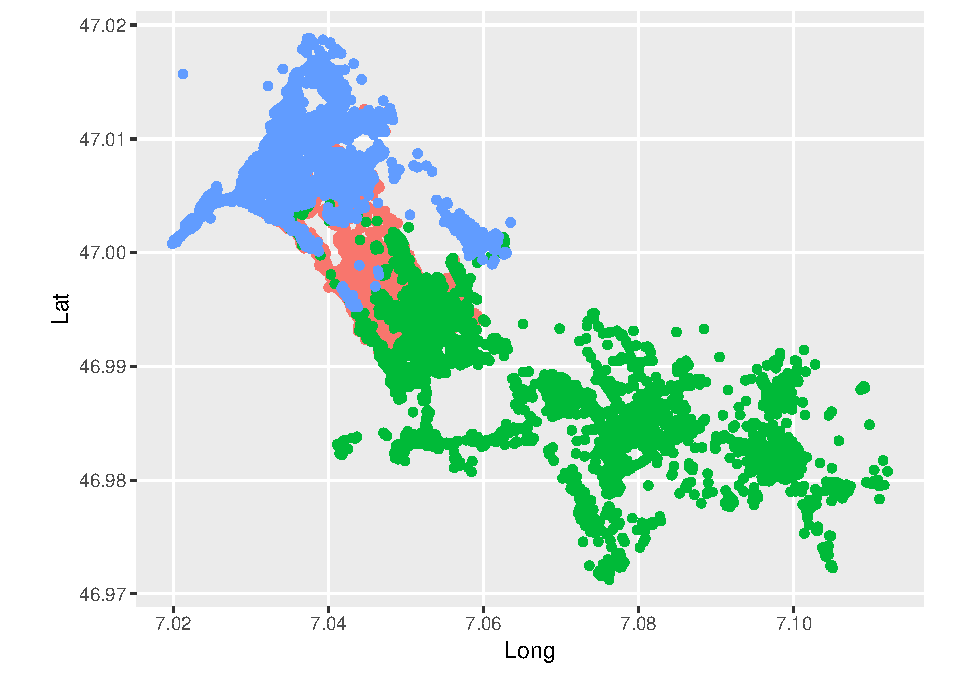
\includegraphics{patterns-and-trends_files/figure-latex/unnamed-chunk-11-1.pdf}

\hypertarget{input-handling-spatial-data}{%
\subsection{Input: Handling spatial data}\label{input-handling-spatial-data}}

Until now, we've stored our location data within data frames as Lat/Long columns. This works well for many tasks, but sometimes we need special \emph{spatial} classes to handle our trajectories. We will get to know such cases in our next tasks, but first we need to convert our \texttt{data.frame} into a spatial object.
Some of you might be familiar with the \texttt{sp} package with the classes \texttt{SpatialPoints}, \texttt{SpatialPointsDataFrame} and so on. These packages are mostly replaced by the fairly new package \texttt{sf}. This packages has some huge advantages over \texttt{sp}:

\begin{itemize}
\tightlist
\item
  simple features are essentially data frames with minor extensions and thus are easily integratable in standard workflows
\item
  they are programmed to cleanly interface with the \texttt{tidyverse} methods (specifically \texttt{dplyr}'s \texttt{mutate} and \texttt{summarise})
\item
  comply with the common Open Geospatial Consortium (OGC) standards (ISO 19125-1:2004) and interface with other important spatial tools such as GDAL, PostGIS, GeoJSON and so fourth
\item
  are being rapidly implemented in visualisation tools such as \texttt{ggplot2}, \texttt{plotly} and \texttt{tmap}
\end{itemize}

We will largely rely on \texttt{sf}when working with vector data in \texttt{R}. In order to transform our \texttt{data.frame} into an sf object, we need to use the function \texttt{st\_as\_sf()} while specifying the columns storing the coordinates and the coordinate reference system\footnote{At this point, we assume you know what a Coordinate Reference Systems is. Check out \href{https://earthdatascience.org/courses/earth-analytics/spatial-data-r/intro-to-coordinate-reference-systems/}{this link} if this is not the case.}.

\begin{Shaded}
\begin{Highlighting}[]
\KeywordTok{library}\NormalTok{(sf)}

\NormalTok{wildschwein_BE_sf <-}\StringTok{ }\KeywordTok{st_as_sf}\NormalTok{(wildschwein_BE, }\DataTypeTok{coords =} \KeywordTok{c}\NormalTok{(}\StringTok{"Long"}\NormalTok{, }\StringTok{"Lat"}\NormalTok{), }\DataTypeTok{crs =} \DecValTok{4326}\NormalTok{)}
\end{Highlighting}
\end{Shaded}

Notice how \texttt{st\_as\_sf} takes the EPSG code for the \texttt{crs\ =} argument. This is so much easier and more elegant than using \texttt{PROJ.4} or \texttt{WKT}. You can find a lot of useful information on Coordinate Reference Systems (including EPSG Codes , etc.) under \href{http://spatialreference.org/ref/epsg/2056/}{spatialreference.org} or \url{http://epsg.io}.

Let's compare our original \texttt{data.frame} with this new \texttt{sf} object:

\begin{Shaded}
\begin{Highlighting}[]
\NormalTok{wildschwein_BE}
\end{Highlighting}
\end{Shaded}

\begin{verbatim}
## # A tibble: 51,246 x 6
##    TierID TierName CollarID DatetimeUTC           Lat  Long
##    <chr>  <chr>       <dbl> <dttm>              <dbl> <dbl>
##  1 002A   Sabi        12275 2014-08-22 21:00:12  47.0  7.05
##  2 002A   Sabi        12275 2014-08-22 21:15:16  47.0  7.05
##  3 002A   Sabi        12275 2014-08-22 21:30:43  47.0  7.05
##  4 002A   Sabi        12275 2014-08-22 21:46:07  47.0  7.05
##  5 002A   Sabi        12275 2014-08-22 22:00:22  47.0  7.05
##  6 002A   Sabi        12275 2014-08-22 22:15:10  47.0  7.05
##  7 002A   Sabi        12275 2014-08-22 22:30:13  47.0  7.05
##  8 002A   Sabi        12275 2014-08-22 22:45:11  47.0  7.05
##  9 002A   Sabi        12275 2014-08-22 23:00:27  47.0  7.05
## 10 002A   Sabi        12275 2014-08-22 23:15:41  47.0  7.05
## # ... with 51,236 more rows
\end{verbatim}

\begin{Shaded}
\begin{Highlighting}[]
\NormalTok{wildschwein_BE_sf}
\end{Highlighting}
\end{Shaded}

\begin{verbatim}
## Simple feature collection with 51246 features and 4 fields
## geometry type:  POINT
## dimension:      XY
## bbox:           xmin: 7.019889 ymin: 46.97125 xmax: 7.112075 ymax: 47.01882
## epsg (SRID):    4326
## proj4string:    +proj=longlat +datum=WGS84 +no_defs
## # A tibble: 51,246 x 5
##    TierID TierName CollarID DatetimeUTC                    geometry
##    <chr>  <chr>       <dbl> <dttm>                      <POINT [°]>
##  1 002A   Sabi        12275 2014-08-22 21:00:12 (7.049618 46.99317)
##  2 002A   Sabi        12275 2014-08-22 21:15:16 (7.049509 46.99416)
##  3 002A   Sabi        12275 2014-08-22 21:30:43 (7.049406 46.99383)
##  4 002A   Sabi        12275 2014-08-22 21:46:07 (7.049217 46.99375)
##  5 002A   Sabi        12275 2014-08-22 22:00:22 (7.049359 46.99375)
##  6 002A   Sabi        12275 2014-08-22 22:15:10 (7.049363 46.99382)
##  7 002A   Sabi        12275 2014-08-22 22:30:13 (7.049326 46.99387)
##  8 002A   Sabi        12275 2014-08-22 22:45:11 (7.049237 46.99395)
##  9 002A   Sabi        12275 2014-08-22 23:00:27 (7.048383 46.99481)
## 10 002A   Sabi        12275 2014-08-22 23:15:41 (7.049396 46.99373)
## # ... with 51,236 more rows
\end{verbatim}

As you can see, \texttt{st\_as\_sf()} has added some metadata to our dataframe (\texttt{geometry\ type}, \texttt{dimension}, \texttt{bbox}, \texttt{epsg} and \texttt{proj4string}) and replaced the columns \texttt{Lat} and \texttt{Long} with a column named \texttt{geometry}. Other than that, the new \texttt{sf} object is very similar to our original dataframe. In fact, \texttt{sf} objects \emph{are} essentially \texttt{dataframes}, just ask \texttt{R}:

\begin{Shaded}
\begin{Highlighting}[]
\KeywordTok{is.data.frame}\NormalTok{(wildschwein_BE_sf)}
\CommentTok{## [1] TRUE}
\end{Highlighting}
\end{Shaded}

All operations we know from handling \texttt{data.frames} can be used on the \texttt{sf} object. Try some out!

\begin{Shaded}
\begin{Highlighting}[]
\CommentTok{# subset rows}
\NormalTok{wildschwein_BE_sf[}\DecValTok{1}\OperatorTok{:}\DecValTok{10}\NormalTok{,]}
\NormalTok{wildschwein_BE_sf[wildschwein_BE_sf}\OperatorTok{$}\NormalTok{TierName }\OperatorTok{==}\StringTok{ "Sabi"}\NormalTok{,]}

\CommentTok{# subset colums}
\NormalTok{wildschwein_BE_sf[,}\DecValTok{2}\OperatorTok{:}\DecValTok{3}\NormalTok{]}
\end{Highlighting}
\end{Shaded}

Instead of keeping the same data twice (once as a \texttt{data.frame}, and once as an \texttt{sf} object), we will overwrite the \texttt{data.frame} and continue working with the \texttt{sf} object from now on. This saves some memory space in \texttt{R} and avoids confusion.

\begin{Shaded}
\begin{Highlighting}[]
\NormalTok{wildschwein_BE =}\StringTok{ }\KeywordTok{st_as_sf}\NormalTok{(wildschwein_BE, }\DataTypeTok{coords =} \KeywordTok{c}\NormalTok{(}\StringTok{"Long"}\NormalTok{, }\StringTok{"Lat"}\NormalTok{), }\DataTypeTok{crs =} \DecValTok{4326}\NormalTok{)}

\KeywordTok{rm}\NormalTok{(wildschwein_BE_sf) }\CommentTok{# we can remove this sf object, since it just eats up our memory}
\end{Highlighting}
\end{Shaded}

\hypertarget{task-4-project-data-from-wgs84}{%
\subsection{Task 4: Project data from WGS84}\label{task-4-project-data-from-wgs84}}

So what can we do with our new \texttt{sf} object that we couldn't before? One example is projecting the WGS84 (\texttt{Lat}/\texttt{Long}) coordinates into the new Swiss CRS \texttt{CH1903+\ LV95}\footnote{As we've mentioned in the first Input, you can look up the EPSG codes under \href{http://spatialreference.org/ref/epsg/2056/}{spatialreference.org} or \url{http://epsg.io}. For information specific to Switzerland, check the \href{https://www.swisstopo.admin.ch/en/knowledge-facts/surveying-geodesy/reference-systems.html}{swisstopo website}}. Do this by using the function \texttt{st\_transform}. By the way, do you notice a pattern here? The package \texttt{sf} names most functions for spatial operations with the prefix \texttt{st\_*}, just as in PostGIS.

Here's the resulting \texttt{sf} object from the operation:

\begin{verbatim}
## Simple feature collection with 51246 features and 4 fields
## geometry type:  POINT
## dimension:      XY
## bbox:           xmin: 2568153 ymin: 1202306 xmax: 2575154 ymax: 1207609
## epsg (SRID):    2056
## proj4string:    +proj=somerc +lat_0=46.95240555555556 +lon_0=7.439583333333333 +k_0=1 +x_0=2600000 +y_0=1200000 +ellps=bessel +towgs84=674.374,15.056,405.346,0,0,0,0 +units=m +no_defs
## # A tibble: 51,246 x 5
##    TierID TierName CollarID DatetimeUTC                  geometry
##    <chr>  <chr>       <dbl> <dttm>                    <POINT [m]>
##  1 002A   Sabi        12275 2014-08-22 21:00:12 (2570409 1204752)
##  2 002A   Sabi        12275 2014-08-22 21:15:16 (2570402 1204863)
##  3 002A   Sabi        12275 2014-08-22 21:30:43 (2570394 1204826)
##  4 002A   Sabi        12275 2014-08-22 21:46:07 (2570379 1204817)
##  5 002A   Sabi        12275 2014-08-22 22:00:22 (2570390 1204818)
##  6 002A   Sabi        12275 2014-08-22 22:15:10 (2570390 1204825)
##  7 002A   Sabi        12275 2014-08-22 22:30:13 (2570387 1204831)
##  8 002A   Sabi        12275 2014-08-22 22:45:11 (2570381 1204840)
##  9 002A   Sabi        12275 2014-08-22 23:00:27 (2570316 1204935)
## 10 002A   Sabi        12275 2014-08-22 23:15:41 (2570393 1204815)
## # ... with 51,236 more rows
\end{verbatim}

\hypertarget{input-calculate-convex-hull}{%
\subsection{Input: Calculate Convex Hull}\label{input-calculate-convex-hull}}

Transforming from one Coordinate Reference System to another was one operation where we needed an object with a spatial nature. In this way, we were able to use an off the shelf function to project the coordinates from one CRS to another. In our next example, we again rely on a spatial function: We want to calculate a \href{https://en.wikipedia.org/wiki/Convex_hull}{convex hull} per Wild boar. And guess what the function for calculating a convex hull is called in \texttt{sf}? If you guessed \texttt{st\_convex\_hull()}, you were right!

By default \texttt{st\_convex\_hull()} calculates the convex hull \emph{per feature}, i.e. \emph{per point} in our dataset. This of course makes little sense. In order to calculate the convex hull per animal, we need to convert our point- to multipoint-features where each feature contains all positions of one animal. This is achieved in two steps:

First: add a grouping variable to the \texttt{sf} object. Note the new grouping variable in the metadata of the \texttt{sf} object. Other than that, \texttt{group\_by} has no effect on our \texttt{sf} object.

\begin{Shaded}
\begin{Highlighting}[]
\NormalTok{wildschwein_BE_grouped <-}\StringTok{ }\KeywordTok{group_by}\NormalTok{(wildschwein_BE,TierID)}

\NormalTok{wildschwein_BE_grouped}
\CommentTok{## Simple feature collection with 51246 features and 4 fields}
\CommentTok{## geometry type:  POINT}
\CommentTok{## dimension:      XY}
\CommentTok{## bbox:           xmin: 2568153 ymin: 1202306 xmax: 2575154 ymax: 1207609}
\CommentTok{## epsg (SRID):    2056}
\CommentTok{## proj4string:    +proj=somerc +lat_0=46.95240555555556 +lon_0=7.439583333333333 +k_0=1 +x_0=2600000 +y_0=1200000 +ellps=bessel +towgs84=674.374,15.056,405.346,0,0,0,0 +units=m +no_defs}
\CommentTok{## # A tibble: 51,246 x 5}
\CommentTok{## # Groups:   TierID [3]}
\CommentTok{##    TierID TierName CollarID DatetimeUTC                  geometry}
\CommentTok{##    <chr>  <chr>       <dbl> <dttm>                    <POINT [m]>}
\CommentTok{##  1 002A   Sabi        12275 2014-08-22 21:00:12 (2570409 1204752)}
\CommentTok{##  2 002A   Sabi        12275 2014-08-22 21:15:16 (2570402 1204863)}
\CommentTok{##  3 002A   Sabi        12275 2014-08-22 21:30:43 (2570394 1204826)}
\CommentTok{##  4 002A   Sabi        12275 2014-08-22 21:46:07 (2570379 1204817)}
\CommentTok{##  5 002A   Sabi        12275 2014-08-22 22:00:22 (2570390 1204818)}
\CommentTok{##  6 002A   Sabi        12275 2014-08-22 22:15:10 (2570390 1204825)}
\CommentTok{##  7 002A   Sabi        12275 2014-08-22 22:30:13 (2570387 1204831)}
\CommentTok{##  8 002A   Sabi        12275 2014-08-22 22:45:11 (2570381 1204840)}
\CommentTok{##  9 002A   Sabi        12275 2014-08-22 23:00:27 (2570316 1204935)}
\CommentTok{## 10 002A   Sabi        12275 2014-08-22 23:15:41 (2570393 1204815)}
\CommentTok{## # ... with 51,236 more rows}
\end{Highlighting}
\end{Shaded}

Second: use \texttt{summarise()} to ``dissolve'' all points into a mulipoint object.

\begin{Shaded}
\begin{Highlighting}[]
\NormalTok{wildschwein_BE_smry <-}\StringTok{ }\KeywordTok{summarise}\NormalTok{(wildschwein_BE_grouped)}

\NormalTok{wildschwein_BE_smry}
\CommentTok{## Simple feature collection with 3 features and 1 field}
\CommentTok{## geometry type:  MULTIPOINT}
\CommentTok{## dimension:      XY}
\CommentTok{## bbox:           xmin: 2568153 ymin: 1202306 xmax: 2575154 ymax: 1207609}
\CommentTok{## epsg (SRID):    2056}
\CommentTok{## proj4string:    +proj=somerc +lat_0=46.95240555555556 +lon_0=7.439583333333333 +k_0=1 +x_0=2600000 +y_0=1200000 +ellps=bessel +towgs84=674.374,15.056,405.346,0,0,0,0 +units=m +no_defs}
\CommentTok{## # A tibble: 3 x 2}
\CommentTok{##   TierID                                                           geometry}
\CommentTok{## * <chr>                                                    <MULTIPOINT [m]>}
\CommentTok{## 1 002A   (2568903 1206200, 2568925 1206207, 2568980 1206197, 2569024 12063~}
\CommentTok{## 2 016A   (2569231 1205823, 2569245 1205925, 2569247 1206027, 2569251 12058~}
\CommentTok{## 3 018A   (2568153 1205611, 2568155 1205613, 2568161 1205624, 2568162 12056~}
\end{Highlighting}
\end{Shaded}

Now we can run \texttt{st\_convex\_hull} on the new \texttt{sf} object.

\begin{Shaded}
\begin{Highlighting}[]
\NormalTok{mcp <-}\StringTok{ }\KeywordTok{st_convex_hull}\NormalTok{(wildschwein_BE_smry)}
\end{Highlighting}
\end{Shaded}

\hypertarget{task-5-ploting-spatial-objects}{%
\subsection{Task 5: Ploting spatial objects}\label{task-5-ploting-spatial-objects}}

Using base plot to visualize \texttt{sf} objects is easy enough, just try the following code.

\begin{Shaded}
\begin{Highlighting}[]
\KeywordTok{plot}\NormalTok{(mcp)}
\end{Highlighting}
\end{Shaded}

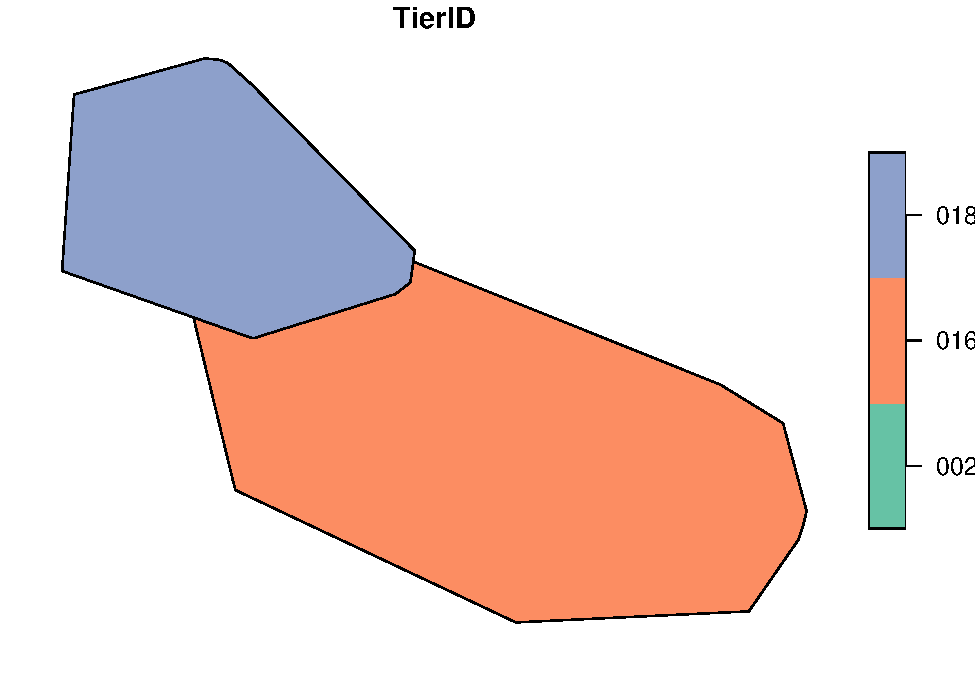
\includegraphics{patterns-and-trends_files/figure-latex/unnamed-chunk-30-1.pdf}

But since we use \texttt{ggplot} extensively, try and plot the object \texttt{mcp} with \texttt{ggplot}. Hint: Use the layer \texttt{geom\_sf()} to add an \texttt{sf} object.

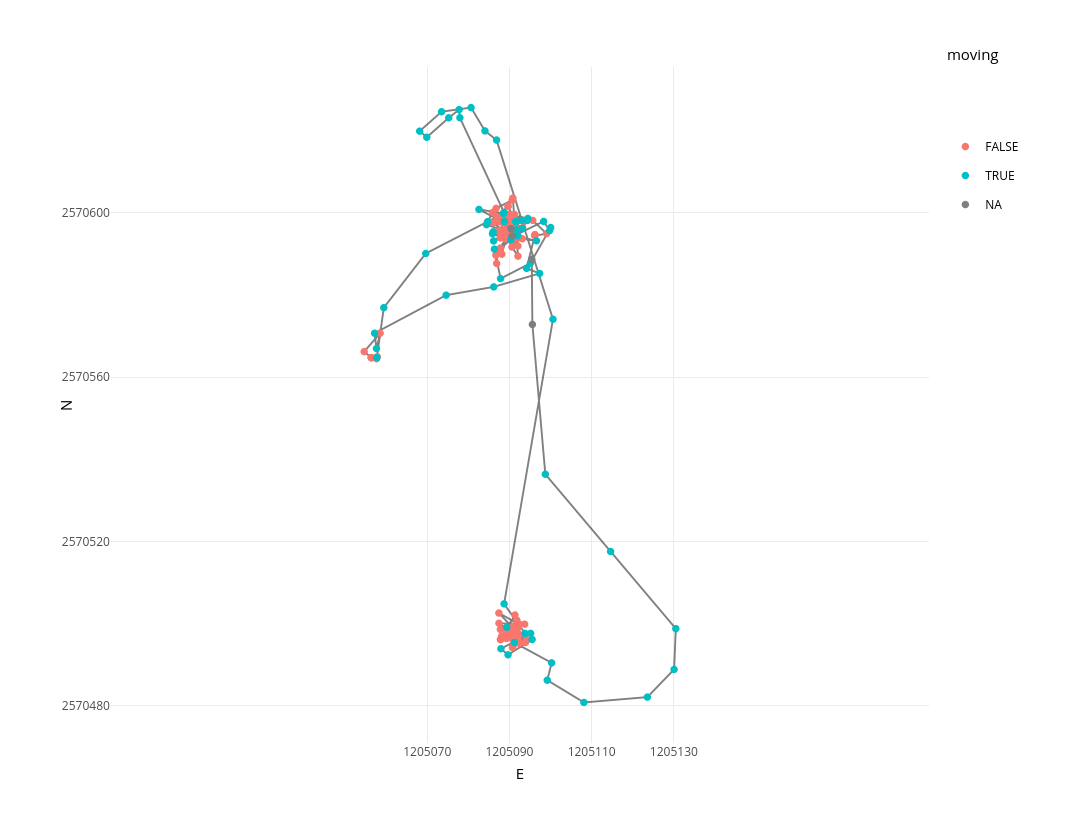
\includegraphics{patterns-and-trends_files/figure-latex/unnamed-chunk-31-1.pdf}

Note: \texttt{ggplot} refuses to use our specified CRS, so we need to force this by specifying \texttt{datum\ =} in \texttt{coord\_sf()}. Try it out.

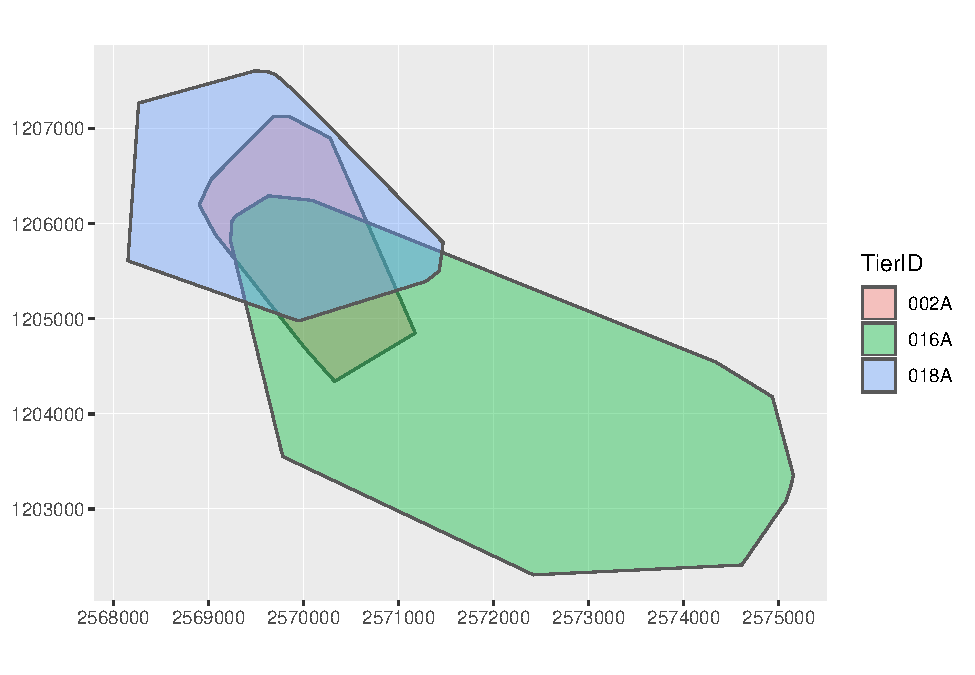
\includegraphics{patterns-and-trends_files/figure-latex/unnamed-chunk-32-1.pdf}

\hypertarget{input-importing-raster-data}{%
\subsection{Input: Importing raster data}\label{input-importing-raster-data}}

In the next task, we would like to add a background map to our \texttt{mcp} object. To do this, we have to the raster data into \texttt{R} first. For this, we use the package \texttt{raster} with the function \texttt{brick}.

\begin{Shaded}
\begin{Highlighting}[]

\KeywordTok{library}\NormalTok{(raster)}

\NormalTok{pk100_BE <-}\StringTok{ }\KeywordTok{brick}\NormalTok{(}\StringTok{"00_Rawdata/pk100_BE_2056.tif"}\NormalTok{)}

\NormalTok{pk100_BE}
\CommentTok{## class      : RasterBrick }
\CommentTok{## dimensions : 1821, 2321, 4226541, 4  (nrow, ncol, ncell, nlayers)}
\CommentTok{## resolution : 5, 5  (x, y)}
\CommentTok{## extent     : 2567000, 2578605, 1199996, 1209101  (xmin, xmax, ymin, ymax)}
\CommentTok{## crs        : +proj=somerc +lat_0=46.95240555555556 +lon_0=7.439583333333333 +k_0=1 +x_0=2600000 +y_0=1200000 +ellps=bessel +towgs84=674.374,15.056,405.346,0,0,0,0 +units=m +no_defs }
\CommentTok{## source     : /home/staff/bako/unix/Lehre/Master/Pattends_and_Trends/Unterrichtsunterlagen_FS2020/00_Rawdata/pk100_BE_2056.tif }
\CommentTok{## names      : pk100_BE_2056.1, pk100_BE_2056.2, pk100_BE_2056.3, pk100_BE_2056.4 }
\CommentTok{## min values :               0,               0,               0,               0 }
\CommentTok{## max values :             255,             255,             255,             255}
\end{Highlighting}
\end{Shaded}

\texttt{pk100\_BE\_2056.tif} is a three layered geotiff File. The above console output shows some metadata including the resolution, extent and the names of our layers (\texttt{pk100\_BE\_2056.1}, \texttt{pk100\_BE\_2056.2}etc). For some reason, \texttt{RasterBrick} imported a fourth layer (\texttt{pk100\_BE\_2056.4}). \texttt{plot()} shows that the fourth layer is empty. We will remove this layer using \texttt{subset()}.

\begin{Shaded}
\begin{Highlighting}[]

\KeywordTok{plot}\NormalTok{(pk100_BE)}
\end{Highlighting}
\end{Shaded}

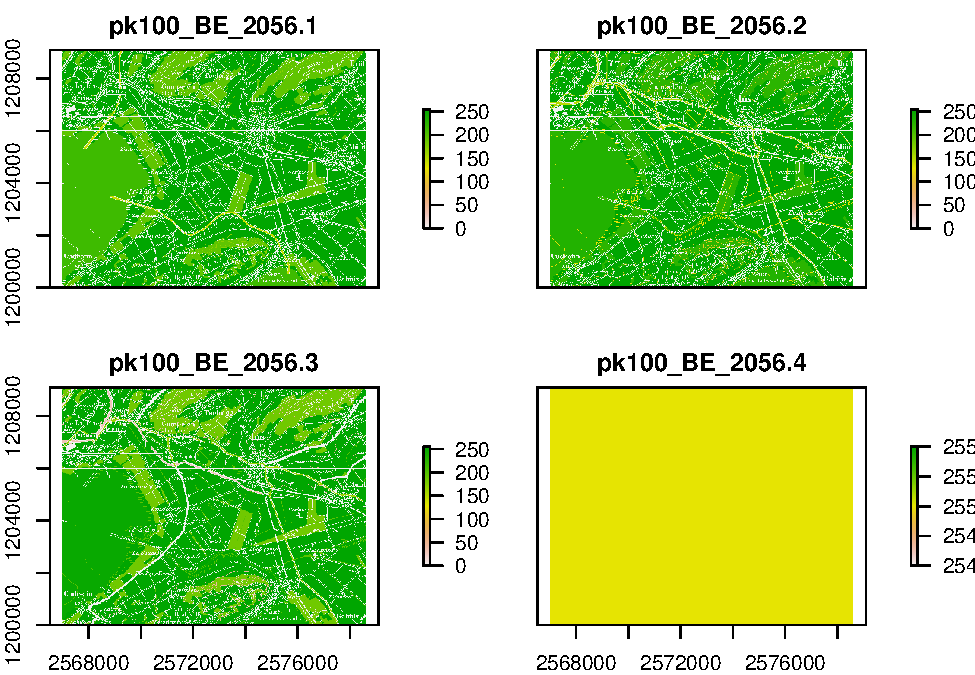
\includegraphics{patterns-and-trends_files/figure-latex/unnamed-chunk-36-1.pdf}

\begin{Shaded}
\begin{Highlighting}[]

\NormalTok{pk100_BE <-}\StringTok{ }\KeywordTok{subset}\NormalTok{(pk100_BE,}\DecValTok{1}\OperatorTok{:}\DecValTok{3}\NormalTok{)}

\KeywordTok{plot}\NormalTok{(pk100_BE)}
\end{Highlighting}
\end{Shaded}

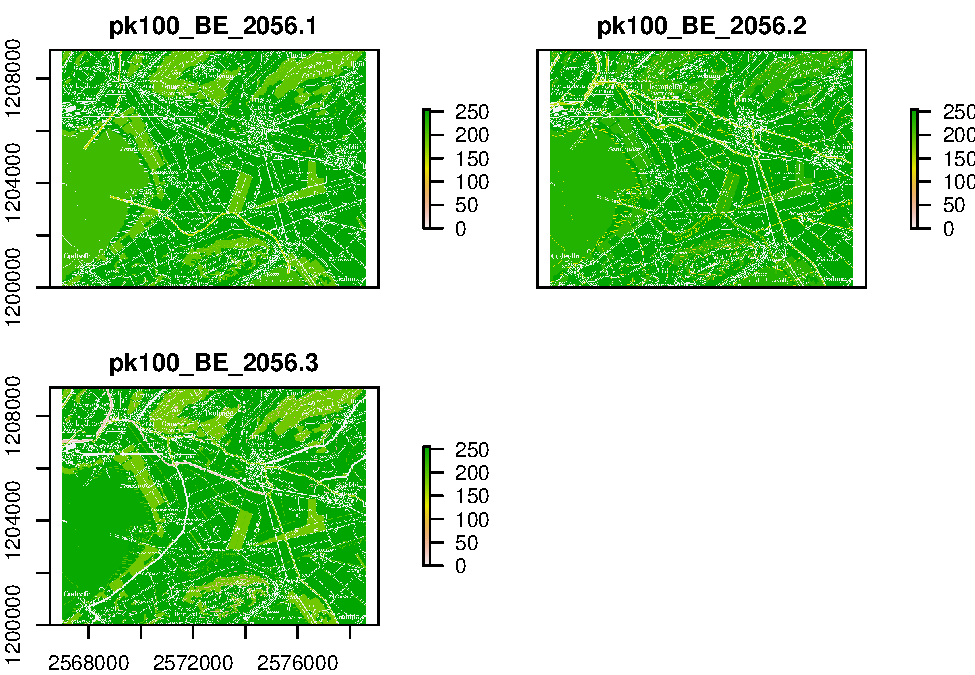
\includegraphics{patterns-and-trends_files/figure-latex/unnamed-chunk-36-2.pdf}

\hypertarget{task-6-adding-a-background-map}{%
\subsection{Task 6: Adding a background map}\label{task-6-adding-a-background-map}}

There are multiple ways to add a background map in \texttt{ggplot}, many require additional packages. This is a good opportunity to get to know a completely different package for creating maps: \texttt{tmap} (``thematic map''). This package was developed with a syntax very similar to \texttt{ggplot2}, which makes it easy to learn.

\begin{Shaded}
\begin{Highlighting}[]
\KeywordTok{library}\NormalTok{(tmap)}


\KeywordTok{tm_shape}\NormalTok{(pk100_BE) }\OperatorTok{+}\StringTok{ }
\StringTok{  }\KeywordTok{tm_rgb}\NormalTok{() }
\end{Highlighting}
\end{Shaded}

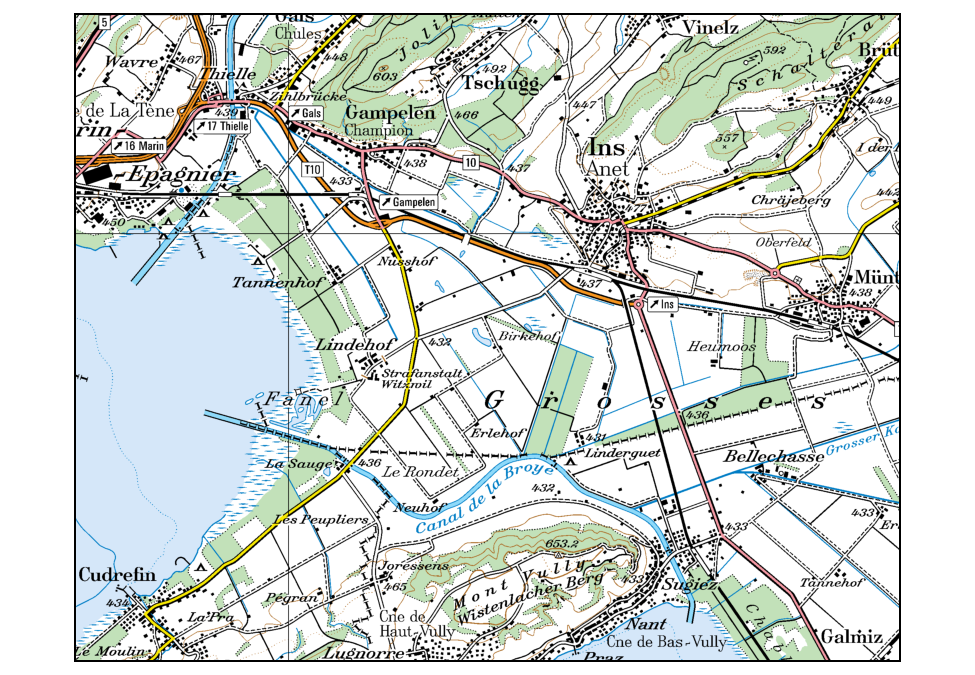
\includegraphics{patterns-and-trends_files/figure-latex/unnamed-chunk-39-1.pdf}

As you can see, plotting layers in \texttt{tmap} is combined with the \texttt{+} sign, just as in \texttt{ggplot2}. In \texttt{tmap} however, each layer consists of two objects: a \texttt{tm\_shape()} in which the data is called, and a \texttt{tm\_*} object in which we define how the data is visualized (\texttt{tm\_rgb()} states that it is plotted as an RGB Raster Layer). Add the object \texttt{mcp} to the plot in this manner. Read \href{https://cran.r-project.org/web/packages/tmap/vignettes/tmap-getstarted.html}{the vignette} if you are having trouble.

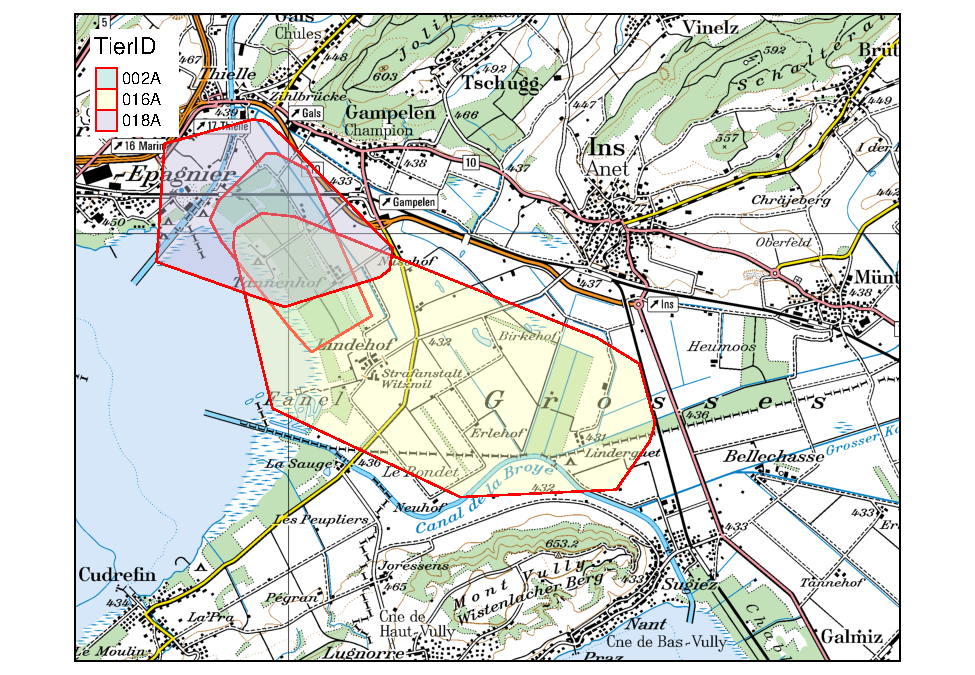
\includegraphics{patterns-and-trends_files/figure-latex/unnamed-chunk-40-1.pdf}

\hypertarget{task-7-create-an-interactive-map}{%
\subsection{Task 7: Create an interactive map}\label{task-7-create-an-interactive-map}}

Rerun the \texttt{tmap()...} command from the previous task, but switch the plotting mode to ``view''" (\texttt{tmap\_mode("view")}) beforehand. Omit the raster layer (\texttt{pk100\_BE}), you won't be needing it.

\hypertarget{references}{%
\chapter*{References}\label{references}}
\addcontentsline{toc}{chapter}{References}

\hypertarget{refs}{}
\leavevmode\hypertarget{ref-wickham2017}{}%
Wickham, Hadley, and Garrett Grolemund. 2017. \emph{R for Data Science: Import, Tidy, Transform, Visualize, and Model Data}. 1st ed. O'Reilly Media, Inc.


\end{document}
